\section{W6: State machines}
State machine is a behaviour model that captures the dynamic behaviour of an object in terms of states, events and state transitions.
\textbf{State:} is the condition of an object at a moment in time.
\textbf{Event:} is a significant or noteworthy occurrence that affects the object to change state.
\textbf{Transition:} is a directed relationship between two states such that an event can cause the object to change from the prior state to the subsequent state.
\textbf{Guard condition:} is a boolean expression that must be true for the transition to occur.
\textbf{Action:} is an operation that is performed when a transition occurs.
\textbf{State-dependent object:} reacts differently to events depending on the object's state.
\textbf{State-independent object:} for all events of interest, an object always reacts to the event the same way.
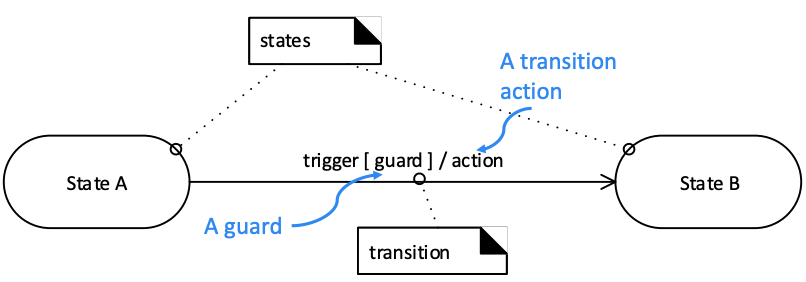
\includegraphics[width=\linewidth]{figs/state-machine.png}
\textbf{Nested state machine:} a state machine that is nested inside another state machine. These are called superstates and substates.
\textbf{Choice pseudostate:} a pseudostate that chooses between two or more transitions.
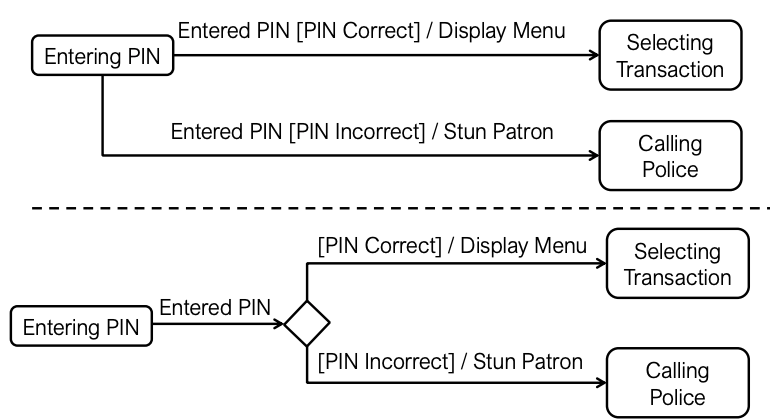
\includegraphics[width=\linewidth]{figs/choice-pseudostate.png}
